\pagestyle{fancy}
\headheight 20pt
\lhead{Ph.D. Thesis --- R. Woods}
\rhead{McMaster - Physics \& Astronomy}
\chead{}
\lfoot{}
\cfoot{\thepage}
\rfoot{}
\renewcommand{\headrulewidth}{0.1pt}
\renewcommand{\footrulewidth}{0.1pt}

\chapter{Radiative Transfer}
\label{chap:radtransfer}

\thispagestyle{fancy}

This chapter will contain an overview of current radiative transfer methods and where we stand.

\section{The Radiative Transfer Problem}
\label{sec:rtformulation}

When considering the transfer of photons, we must consider the scale we are dealing with. At the individual photon level, propagation is described by classical electrodynamics. Once we get to larger scales, however, it is more useful to treat radiation in ``packets'' or as an energy flux.

Consider an infinitesimal patch of area, dA, normal to a direction $\hat{n}$. We consider an infinitesimal solid angle, $d\Omega$, and consider all rays passing through the area and within the solid angle (see figure \ref{fig:intensity}).

\begin{figure}
\label{fig:intensity}
\includegraphics[width=\textwidth]{graphics/placeholder.eps}
\caption{The geometry for all rays at a point p through area dA within solid angle $d\Omega$.}
\end{figure}

The energy through this area patch, within the solid angle, in time dt, and within the frequency range $d\nu$ is

\begin{equation}
\label{eq:intensity}
dE = I_{\nu}dA dt d\Omega d\nu,
\end{equation}

where $I_{\nu}$ is \emph{specific intensity} (specific because it is within a frequency range; dropping the frequency dependence makes this intensity). Specific intensity has units of energy per unit area per unit time per unit solid angle per unit frequency. It is useful to consider radiation in terms of intensity because it enables a macroscopic description of radiation that includes microscopic effects like scattering and absorption.

We can recover familiar values such as flux (or pressure or density) by taking moments of the intensity,

\begin{equation}
\label{eq:flux}
F_{\nu} = \int I_{\nu}\cos{\theta}d\Omega,
\end{equation}

where $F_{\nu}$ is the specific flux (flux at a particular wavelength).

Let us now consider the passage of these rays through some matter. If we consider a ray, then energy may be added or removed from this ray due to absorption (removing photons), emission from the matter (adding photons), or scattering (scattering into or out of the ray). We first consider emission.

We define the specific (monochromatic) emission emission coefficient, j, as the energy emitted per unit time, per unit solid angle, per unit volume, and per unit frequency,

\begin{equation}
\label{eq:emissioncoef}
dE = j_{\nu} dV dt d\Omega d\nu.
\end{equation}

If we trace along a ray with cross section dA some distance ds, it will cover a volume of $dV = dA ds$. Since equation \ref{eq:emissioncoef} and equation \ref{eq:intensity} only differ by a factor of distance (dA compared to dV), we can find the change intensity along the beam due to emission as

\begin{equation}
\label{eq:emissionintensity}
dI = j_{\nu} ds.
\end{equation}

Equation \ref{eq:emissionintensity} describes the amount of intensity added to a ray along some path ds due to spontaneous emission. If emission were the only process to worry about, finding intensity would be a simple matter of integrating the equation. [However, we must consider other physical processes for a more complete description.]

We next consider absorption. Consider again a ray traveling along a path ds. The amount of intensity lost due to absorption can be defined as

\begin{equation}
\label{eq:absorption}
dI = -\alpha I ds,
\end{equation}

where $\alpha$ is called the absorption coefficient and has units of distance$^{-1}$. It can be shown \citep{rybickiLightman86} that $\alpha$ is a function of more commonly known variables,

\begin{equation}
\label{eq:absorptioncoeff}
\alpha = -n \sigma I ds = -\rho \kappa I ds
\end{equation}

where n is the number density of particles, $\sigma$ is the cross section (in units of distance squared) of each absorbing particle, $\rho$ is the mass density, and $\kappa$ is the opacity (in units of distance squared per unit mass). Notice that the only difference between $n \sigma$ and $\rho \kappa$ is the average mass of the absorbing particles. Note that our algorithm has chosen to use $\rho$ and $\kappa$.

Finally, we consider scattering. Scattering is a process that both subtracts and adds to the intensity. We can define a specific emission coefficient for scattering by equating the power per unit volume per frequency emitted to the power received,

\begin{equation}
\label{eq:scatteringcoefficient}
j_{s,\nu} = \sigma_{\nu} J_{\nu},
\end{equation}

where $\sigma_{\nu}$ is the specific scattering coefficient, and $J_{\nu}$ is the specific mean intensity, defined as

\begin{equation}
\label{eq:meanintensity}
J_{\nu} = \frac{1}{4\pi}\int I_{\nu} d\Omega.
\end{equation}

Before combining all of the processes affecting radiative transfer, it is useful to introduce a variable called the specific \emph{Source Function},

\begin{align}
\label{eq:sourcefunction}
S_{a,\nu} &\equiv \frac{j_{\nu}}{\alpha_{\nu}},\\
S_{s,\nu} &\equiv \frac{j_{\nu}}{\alpha_{\nu}}.
\end{align}

The source function is the ratio of emission to absorption and describes the intensity that an object will tend to. In the case of pure absorption, emission is 0 and so the source function is 0, since the intensity would tend to 0. In the case of pure emission, the source function is infinite and intensity tends to infinity since nothing is removing photons.

We now have the base equations to put together a description of radiative transfer that includes the processes of spontaneous emission, absorption, and scattering. Combining equations \ref{eq:emissionintensity}, \ref{eq:absorption}, \ref{eq:scatteringcoefficient}, \ref{eq:meanintensity}, and \ref{eq:sourcefunction}, we can write

\begin{align}
\label{eq:combinedtransfer}
\frac{dI_{\nu}}{ds} &= (-\alpha_{\nu}I_{\nu} + j_{\nu}) - (\sigma_{\nu}I_{\nu} + j_{s,\nu}) \nonumber\\
 &= -\alpha_{\nu}(I_{\nu} - S_{a,\nu}) - \sigma_{\nu}(I_{\nu} - S_{s,\nu}) \nonumber\\
 &= -(\alpha_{\nu} + \sigma_{\nu})(I_{\nu}-S_{\nu}),
\end{align}

where the combined source function $S_{\nu}$ is defined as

\begin{equation}
\label{eq:combinedsourcefunction}
S_{\nu} \equiv \frac{\alpha_{\nu}S_{a,\nu} + \sigma_{\nu}S_{s,\nu}}{\alpha_{\nu} + \sigma_{\nu}}.
\end{equation}

According to equation \ref{eq:scatteringcoefficient}, the source function for scattering is actually mean intensity (equation \ref{eq:meanintensity}), meaning that the above equation is actually an integro-differential equation - it is a function of $I_{\nu}$, $\frac{dI_{\nu}}{ds}$, and $\int I_{\nu} d\Omega$. Thus, any equation involving scattering is significantly more difficult to solve. Numerical solutions to integro-differential equations are usually specialized and complex [cite someone].

For this reason, scattering is often omitted from radiative transfer solver due to very large added computational cost. In this thesis, our solutions do not explicitly account for scattering, though it is possible scattering-like behavior (due to properties of the RT algorithm and the properties of SPH) may result in some solutions [remove this line I think].

If scattering is omitted, equation \ref{eq:combinedtransfer} is simplified to a nicer form. We combine equations \ref{eq:emissionintensity}, \ref{eq:absorption}, and \ref{eq:sourcefunction} to obtain

\begin{equation}
\label{eq:transferequation_s}
\frac{dI_{\nu}}{ds} = -\alpha_{\nu}I_{\nu} + j_{\nu}.
\end{equation}

It is now useful to introduce optical depth $\tau_{\nu}$,

\begin{equation}
\label{eq:opticaldepth}
\tau(s) = \int_{s_0}^{s} \alpha_{\nu}(s')ds' = \int_{s_0}^{s} \reveryho(s') \kappa_{\nu}(s') ds'.
\end{equation}

Optical depth is a unitless value that describes the mean free path of a photon between interactions. The distance needed in the integral to give $\tau_{\nu} = 1$ should correspond to one mean free path given the absorption coefficient $\alpha_{\nu}$. It is useful to rewrite equation \ref{eq:transferequation_s} in terms of $\tau_{\nu}$ and $S_{\nu}$ by simply dividing by $\alpha_{\nu}$

\begin{equation}
\label{eq:transferequation_t}
\frac{dI_{\nu}}{d\tau_{\nu}} = -I_{\nu} + S_{\nu}.
\end{equation}

Equation \ref{eq:transferequation_t} is the transfer equation for radiation as it is most commonly seen. A solution can be obtained by using an integrating factor of $e^{\tau_{\nu}}$, which gives the formal solution to the transfer equation

\begin{equation}
\label{eq:transferequationsolution}
I_{\nu}(\tau_{\nu}) = I_{\tau}(0)e^{-\tau_{\nu}} + \int_0^{\tau_{\nu}} e^{-(\tau_\nu - \tau'_{\nu})} S_{\nu}(\tau'_{\nu})d\tau'_{\nu}.
\end{equation}

Solving the above equation at a point in a simulation would give you a radiation field that accounted for emission and absorption at all other points in the simulation. This would then be repeated at all points for which a radiation field should be known.

It should now be clear why radiative transfer is a difficult problem; analytically, it involves integrals over source functions that are not necessarily known at all points in space, with both density and opacity varying as a function of position as well. Numerically, we are trying to solve a function of seven variables - three position, two angular, time, and frequency - $I = I(x,y,z,\theta,\phi,t,\nu)$.

[Add further simplifications to the equation here? Just talk about the absorption solution? Mention that integrating over all emission typically amounts to summing over all sources.]

%\begin{equation}
%\label{eq:rademission}
%I(s) = I(s_0) + \int_{s_0}^{s} j(s') ds'
%\end{equation}
%
%\begin{equation}
%\label{eq:radabsorption}
%I(s) = I(s_0)\exp{\left[-\int_{s_0}^{s} \alpha(s') ds'\right]} = I(s_0)\exp{\left[ -\tau (s) \right]}
%\end{equation}

\section{Current Methods}
\label{sec:currentmethods}

The equations presented in section \ref{sec:rtformulation} are very difficult to solve if approximations are not made. Seven dimensions means that even if each dimension only has a resolution of 100 elements, we must keep track of $10^14$ elements, or roughly one petabyte of data if each element is 10 bytes. In many cases, 100 elements is not nearly fine enough to resolve important features in a dimension, especially in frequency where many sharp features are present. The problem is already numerically impractical from a memory perspective.

As well, the transfer equation is an integro-differential equation, meaning that common numerical solvers are not useful. Solvers for this type of equation are generally complex and specific purpose, so the actual numerical method side is also difficult.

In order to overcome the above, different approximations to the equation are adopted. Different approximations give rise to different advantages and disadvantages in accuracy and speed and typically apply best to particular regimes.

Current popular strategies include monte-carlo, ray tracing, grid-based solvers, and moment methods. The following sections will give a brief description of each method as well as common properties of the methods.

\subsection{Monte-Carlo Solvers}
\label{montecarlo}

Monte-Carlo methods are perhaps the most obvious way to solve the radiative transfer problem. The most basic solution follows a photon from emission, through any scattering, until it leaves the simulation. At any point during the path, random numbers are used to determine whether the photon will be scattered, what direction it will be scattered, whether it will be absorbed and re-emitted, and what wavelength the re-emitted photon(s) will be.

In practice, following individual photons is not practical. Instead, following ``photon packets'' is more useful. Packets are typically defined as a group of photons [cite codes that do this] or as having a specified energy (in which case, the number of photons can be determined by using $E = h\nu$). The latter choice has the benefit that when re-emission occurs after an absorption at a lower wavelength, there are not now more photons to keep track of. The ray retains the same energy and more photons are implied since $\nu$ changes \citep{ercolanoEt03,abbottLucy85}.

% calculate random distance based on relation between random number and normalized optical depth - harries and howarth 97
% or, ask probability at each new cell that it is absorbed - Lucy 1999.
% first method more expensive - ercolano et al 2003

%estimator is needed - MC provides means to relate quantities we observe to physical quantities we want to determine. Need measure of mean intensity. See eq 9 in ercolano 03 for estimator from Och et al 98. Also create new estimator.

%Emission happens as sampled from local gas spectrum.

%process is iterative. When photons have all been sent, can iterate with estimator from above and local ionization state to converge on values.

%can finally use results to make observations if desired (usually primary use of this method).





%In monte-carlo methods, a photon is carefully tracked through a domain, following scattering, absorption, and re-emission. See [from steinacker 09] \citet{wolf03,woodEt2004,ercolanoEt2005,jonsson06,pinteEt06}. [ADD method basics]

%\begin{itemize}
%\item Advantages - can treat complicated spatial distributions, arbitrary scattering functions, and polarization.
%\item Disadvantages - Very high or low optical depths hard (why?), re-emission in all directions over many events hard (why?), no global error control
%\end{itemize}


\subsection{Ray Tracing}
\label{sec:raytracing}

Ray tracing has the ability to treat arbitrary density distributions, and can use general solvers for ODEs. Fairly accurate and fairly expensive.

\begin{itemize}
\item Often combined with monte-carlo methods
\item Provides quite accurate results.
\item Provides global error control.
\item Can cause step-size limitations in order to consistently transfer photons.
\item Becomes impractical at high optical depth and can require complicated solvers.
\end{itemize}


\subsection{Grid-Based Methods}
\label{sec:gridmethods}

Can use simple solvers (finite differencing or short characteristics) and gives good error control.

\begin{itemize}
\item Grid must be adaptable to be practical, though good refinement criteria is unclear
\item Interpolation between grids can be costly and give interpolation errors.
\item Numerical diffusion typically not taken into account.
\end{itemize}


\subsection{Moment Methods}
\label{sec:momentmethods}

e.g. FLD or M1 moment codes (skinner + ostriker, others). Fairly accurate, faster than ray tracing, in specific regimes.

\begin{itemize}
\item Well suited for optically thick regime (can do free streaming)
\item Struggles with peaked radiation in optical depths of order 1.
\end{itemize}

\subsection{Summary of Methods}
\label{sec:summaryofmethods}


%The current set of computational methods can be classified as follows:
%
%\begin{itemize}
%\item Very accurate, expensive methods - monte carlo, ray tracing
%\item Methods accurate in specific scenarios, e.g. FLD for optically thick, ``str\"omgren method'' from Dale
%\item \emph{Very} rough approximations, e.g. method that only looks at absorption near sink and source.
%\end{itemize}
%
%As will be seen, there is currently an opening in the market for something in the middle - Decent accuracy at a low cost.

